\subsection{Menawar/melelang barang}
Halaman ini hanya dapat diakses oleh pengguna yang sudah terdaftar. Halaman ini menampilkan halaman informasi barang, dan sebuah elemen \textit{input} harga , dan pengguna dapat mengisi lalu mengklik tombol daftar, dan untuk kasus normal dan alternatif dapat dilihat pada Tabel \ref{uc02.03}.\\
\indent Alur pemrosesan dan logika program pada kasus penggunaan ini dapat dijabarkan sebagai berikut:
	\begin{enumerate}
		\item Pemrosesan \textit{back-end} ditulis menggunakan PHP yang dicantumkan dalam Kode Sumber \ref{cdbe.02-03}; 
		\item Logika \textit{view} ditulis menggunakan jQuery yang dicantumkan dalam Kode Sumber \ref{cdjq.02-03}; dan
		\item Logika proses lelang, berjalan diatas socket yang berjalan diatas Node.js dengan bantuan Socket.io yang dicantumkan dalam Kode Sumber \ref{cdsoc.02-03}
	\end{enumerate}

\begin{figure}[H]
    \centering
    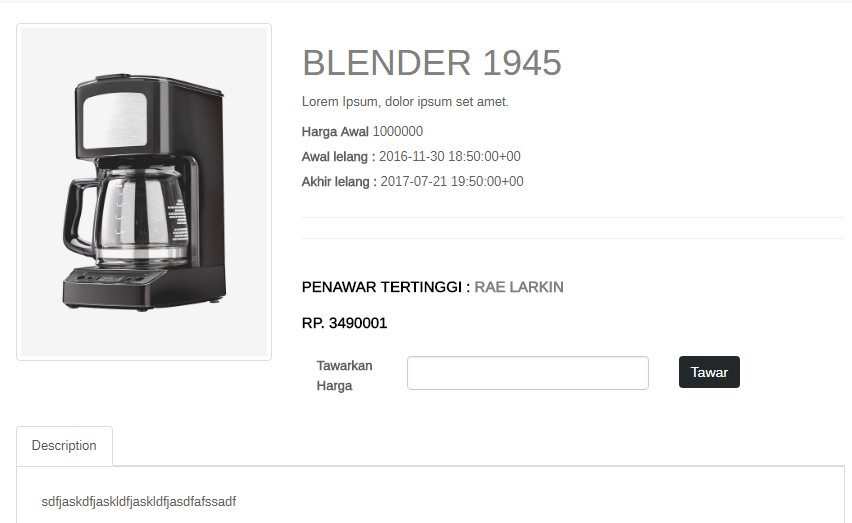
\includegraphics[width=\textwidth]{images/bab4/ui/02-03.png}
    \caption{Halaman Antarmuka  Implementasi Kasus Penggunaan Menawar/melelang barang}
    \label{ui.02-03}
\end{figure}

\begin{lstlisting}[label=cdbe.02-03,style=php,caption=Kode Sumber \textit{Back-end} Menampilkan Halaman Lelang Barang]
/*	file : app/Http/Controllers/ItemController*/
public function show($id){
	/*	method : GET */

	/*	tampilkan halaman */
    $data['item'] = $this->itemRep->find($id);
    
    if($data['item']->bid_status == 1 )
    {
        $data['currentPrice'] = $this->itemRep->getCurrentPrice($id);
    }

    /*	Jika barang yang disubmit sudah selesai/dimenangkan,
    	tambahkan variabel winner ke view */
    if($data['item']->bid_status == -1 && $data['item']->winner_chosen_status)
        $data['winnername'] = User::find($data['item']->id_user)->name;

    /*	tampilkan halaman */
    return view('pages.'.$this->pageFolder.'.detail', $data);
}
\end{lstlisting}


\begin{lstlisting}[label=cdsoc.02-03,style=htmlcssjs,caption=Kode Sumber Logika Lelang (menggunakan Node.js)]
/*	
	file : bidserver_https.js 
	menggunakan dependencies : socketio (ioServer), https, http, fs dan express
*/
socket.on('submitbid', function(bidjson) {

    // parameter (bidjson) adalah JSON yang terdiri dari :
    // id_bidder, id_item, dan harga_bid

    var bidobj = JSON.parse(bidjson);
    biddingAPI.submitBid(bidobj, function(status, result)
    {
      //  status adalah return value
      //  jika status = 1, broadcast ke room
      //  untuk mengupdate pemenang lelang saat tersebut.
      if (status=="1")
      {
          //jika sukses
          var messageObject = {};
          var tokenArray;
            
            // fungsi untuk mengconstruct 
            // return message
          constructBroadcastMsg(messageObject);

            // broadcast ke semua yang 
            // join ke room lelang tersebut.
          io.to(result.item_id_return).emit('bidsuccess', result);
        
      }
      else if (status=="0"){
        // jika gagal, 
        // maka send ke sender bahwa bid failed
        socket.emit('bidfailed', { bidstatus: "failed" });
      }
    });

});
\end{lstlisting}

\begin{lstlisting}[label=cdjq.02-03,style=htmlcssjs,caption=Kode Sumber Logika UI (menggunakan jQuery)]
// script ini berjalan
// saat tombol Tawar diklik

$('.tawar').click(function()
{
    var penawaran = $('#submitted_price').val();
    var priceNow = $('.priceongoing').html();
    if(penawaran==""){
        alertNoPriceSubmitted();
    }
    else if(penawaran < priceNow ){
        alertInvalidBid();
    }
    else {
        var JSONToSend;
        constructJson(JSONToSend);

        // submit bid ke socket
        socket.emit('submitbid', JSONToSend);

        // tunggu return dari socket
        // jika hasilnya bid failed, maka tampilkan pesan error
        socket.on('bidfailed', function (result) {
            alertFailedBid();
        });

        // jika hasilnya bid sukses,
        // tampilkan pesan sukses (toast)
        // dan render ulang halaman (ubah isi elemen)
        socket.on('bidsuccess', function (result) {
            alertSuccessfulBid();
            renderPageWithNewPrice(result);
        });
    }
});
\end{lstlisting}


